\documentclass[t]{beamer}
\usetheme{Warsaw}
\usecolortheme{seahorse}
\usepackage{array}
%\usepackage{graphicx}
\usepackage{amssymb,amsmath,mathrsfs,amsfonts}
%\usepackage[colorhighlight,display]{texpower}
%\usepackage{caption}
%\usepackage[all]{xy}
\usepackage{beamerthemesplit}
\mode<presentation>
%\usepackage{pause}
\usepackage{ulem}  % for strikethroughs
\usepackage{cancel} % for strikethroughs in math mode 
\usepackage{tikz}
\usepackage{calc}
\usetikzlibrary{shapes}
\usepackage{hyperref}
\hypersetup{pdfpagemode=FullScreen}
\usepackage{ifthen}
\usepackage{animate}
\usepackage{color}
\usepackage{type1cm}  % used for watermarking
\usepackage{eso-pic}  % used for watermarking


\theoremstyle{plain}
\newtheorem{prop}{Proposition}
\newtheorem{thm}[prop]{Theorem}
\newtheorem{lem}[prop]{Lemma}
\newtheorem{cor}[prop]{Corollary}
\theoremstyle{definition}
\newtheorem{dfn}{Definition}
\newtheorem{rem}[prop]{Remark}
\newtheorem{ex}{Example}[section]
%\newtheorem{note}{Note}[section]
\newtheorem{exercise}{Exercise}[section]
\newcommand{\nin}{\noindent}
\newcommand{\ds}{\displaystyle}
\renewcommand{\figurename}{Figure \arabic{figure}}



\renewcommand*\familydefault{\sfdefault} 




%%%%%%%%%%%%%%%%%%%%%%%%%%5
%%%%%%%%%%%%%%%%%%%%%%%%%%%%
%%%% some commands that have different meaning in the article/presentation modes

\newcommand{\vvfill}{\mode<presentation>{\vfill}  \mode<article>{\medskip}}   %vfill in presentation only
\newcommand{\sketchspace}{ 
\mode<article>{ \medskip\noindent{\textbf{Sketch:}} \vspace*{6cm} }
\mode<presentation>{ } 
}
\newcommand{\examplespace}{ 
\mode<article>{ \medskip\noindent{\textbf{Example:}} \vspace{6cm} }
\mode<presentation>{ } 
}
\newcommand{\artsmspace}{\mode<article>{\vspace*{2cm}} }  %small space in article mode
\newcommand{\artlargespace}{\mode<article>{\vspace*{6cm}} }  %large space in article mode

\newcommand{\dx}{\,dx}

\newcommand{\soln}{{\textbf{Solution: }}\,\,\,}
\newcommand{\disp}{\displaystyle}

\newcommand{\makedate}{\vvfill
\begin{picture}(10,10)  
\put(260,-20){\mbox{\tiny{\today}}}
\end{picture}
}

\newcommand{\pd}[2]{\dfrac{\partial#1}{\partial#2}}
\newcommand{\pD}[2]{\dfrac{\partial^2#1}{\partial#2^2}}
\newcommand{\pdd}[3]{\dfrac{\partial^2#1}{\partial#2 \partial#3}}


\normalem %stops the ulem package making all the emphs into underlines...
 
 
 
 \newcommand{\refandrev}[2]{
 \begin{small}
  \hspace{6cm}
  \begin{minipage}[r]{8cm}
  Stewart,    Chapter #1   \\
  Review:  \parbox[t]{6cm}{#2}
\end{minipage}
\end{small}
}



\newcounter{heading}
\setcounter{section}{1}
\setcounter{heading}{0}

\newcommand{\makeheading}[1]{\medskip\begin{large}\noindent\textbf{{#1}}\end{large}\smallskip}

%\newenvironment{head}[1]{\medskip\stepcounter{heading}\noindent\textbf{\hspace{0.2cm}{#1}.}}{}
\newcommand{\newhead}[1]{\medskip\stepcounter{heading}\noindent\textbf{\hspace{0.2cm}{#1}.}}


\newcommand{\pf}[1]{\noindent\textit{Proof.}\vspace*{#1 cm}}
\newcommand{\sol}[1]{\noindent\textit{Solution.}\vspace*{#1 cm}}
\newcommand{\further}[1]{\begin{small}\noindent\textit{Further reading: #1}\end{small}}
\newcommand{\exr}[1]{\begin{footnotesize}\noindent\textit{\textbf{Exercises:} Stewart #1}\end{footnotesize}}


% Sets of numbers
\newcommand{\C}{\mathbb{C}}
\newcommand{\RR}{\mathbb{R}}
\newcommand{\Z}{\mathbb{Z}}
\newcommand{\N}{\mathbb{N}}
\newcommand{\Q}{\mathbb{Q}}

% Partitions
\newcommand{\PP}{\mathcal{P}}

% Limits
\newcommand{\limm}[1]{\displaystyle \lim_{x\to #1}}

% Backslash
\newcommand{\bs}{\backslash}

% functions
\newcommand{\cosec}{\mathrm{cosec}}
\newcommand{\cosech}{\mathrm{cosech}}
\newcommand{\sech}{\mathrm{sech}}
\newcommand{\Li}{\mathrm{Li}}
\newcommand{\si}{\mathrm{Si}}
\newcommand{\erf}{\mathrm{erf}}

% Domain and Range
\newcommand{\Dom}{\mathrm{Dom}}
\newcommand{\Codom}{\mathrm{Codom}}
\newcommand{\Range}{\mathrm{Ran}}



\title{Week 8: Applications: Area and Average Value}
%\date{September 24 -- September 28, 2012}

\begin{document}

\frame{\titlepage}

\setcounter{tocdepth}{2}
\frame{\tableofcontents

\begin{flushright}
%\hyperlink{tues}{\beamergotobutton{Lecture 14}}
\end{flushright} 
}

\AtBeginSection[]
{
\begin{frame}<beamer> 
\tableofcontents[currentsection]  % show TOC and highlight current section
\end{frame}
}

\section{Area}

\begin{frame}
\footnotesize
\begin{dfn} 
Area between two curves $f(x)$ and $g(x)$, in the interval $[a, b]$ is:

$$ A = \lim_{n\rightarrow \infty} \sum_{i=1}^{n} \left[ f(x_i^{*}) - g(x_i^{*})  \right] \Delta{x}$$

or in a integral form as:

$$ A = \int_{a}^{b} \left[ f(x) - g(x) \right] \, dx $$
\end{dfn}

\begin{figure}[t]
\begin{center}
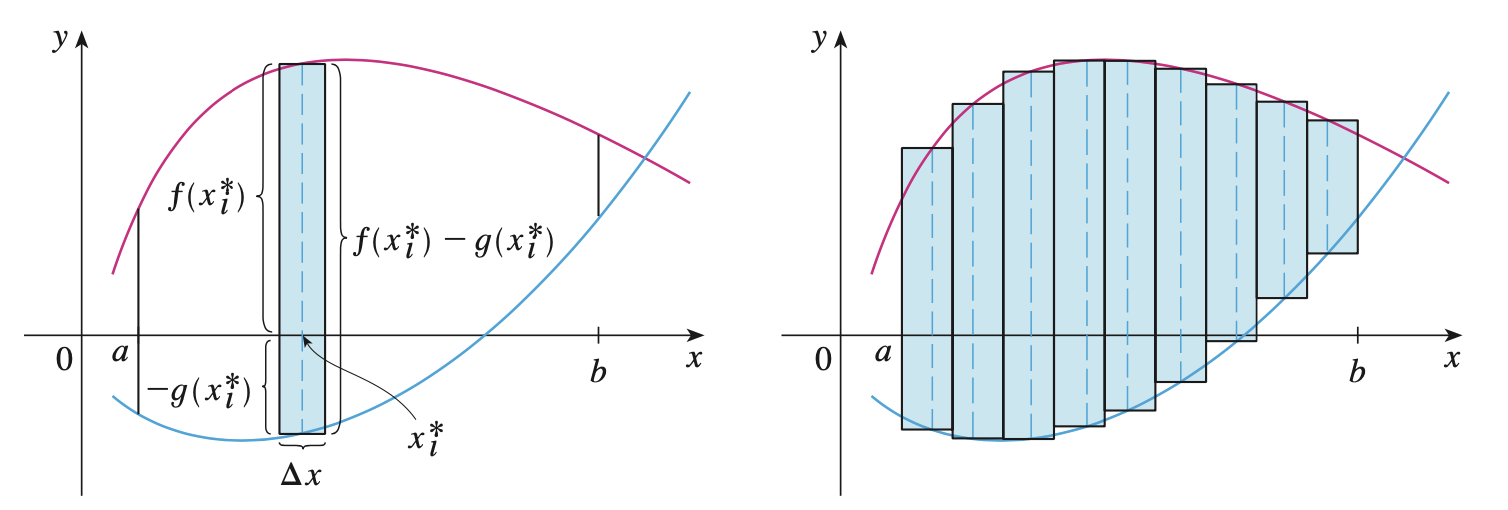
\includegraphics[scale=0.4]{fig/area}
\end{center}
\end{figure}

\end{frame}

\begin{frame}

\frametitle{Use Case: Level of infected cells}

\begin{figure}[t]
\begin{center}
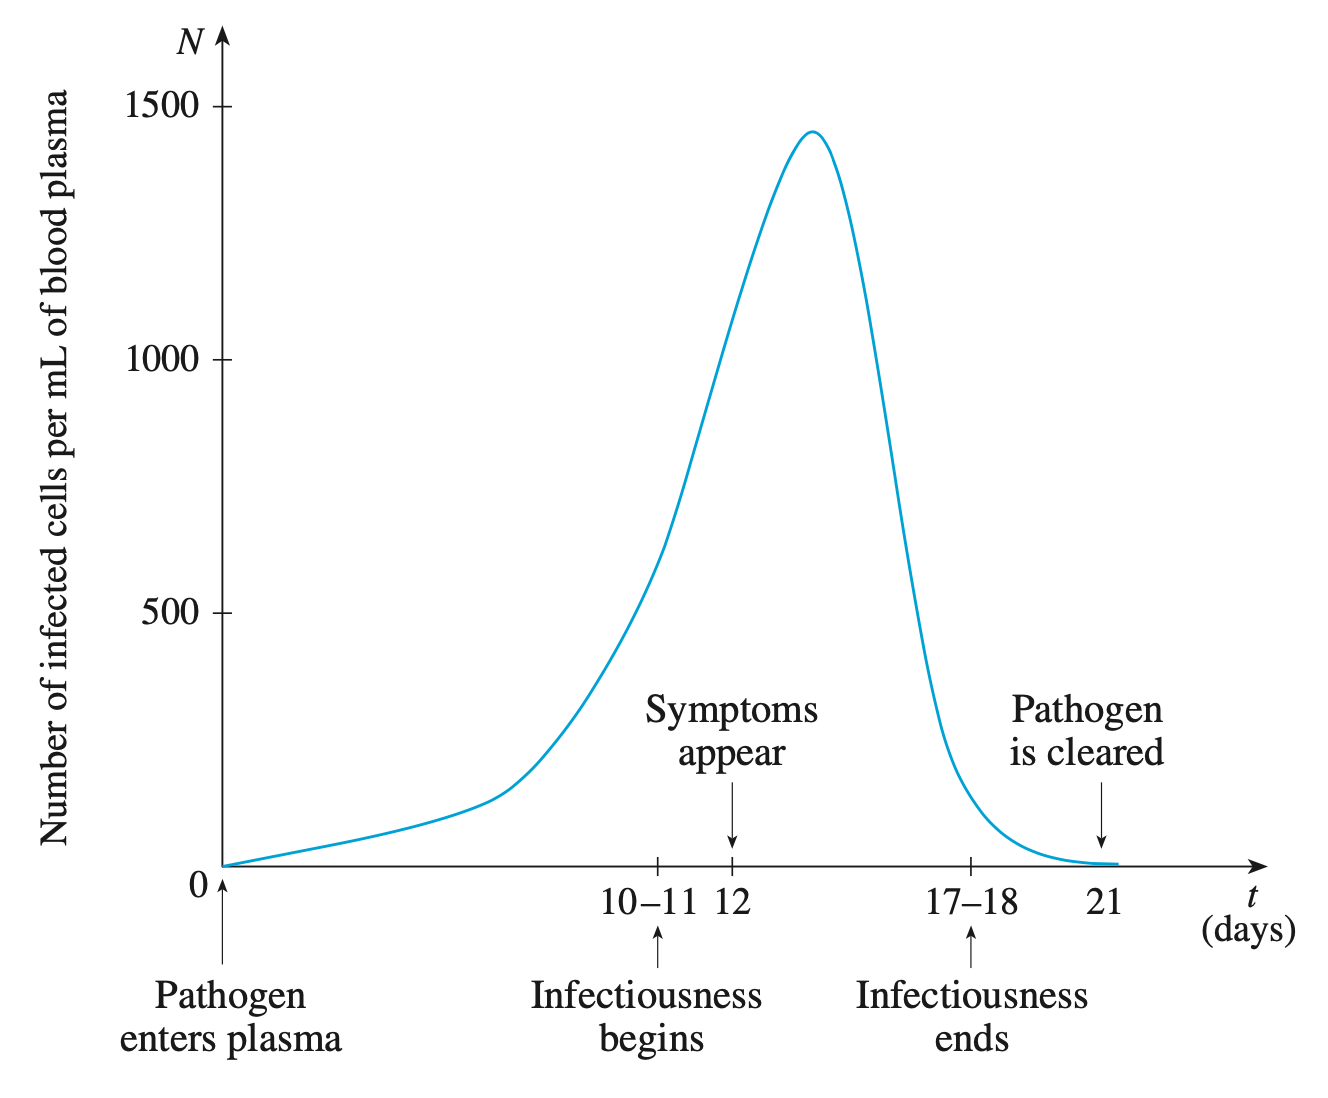
\includegraphics[scale=0.35]{fig/area_case}
\end{center}
\end{figure}

\end{frame}

\begin{frame}

\frametitle{Use Case: Distances between cars}

\begin{figure}[t]
\begin{center}
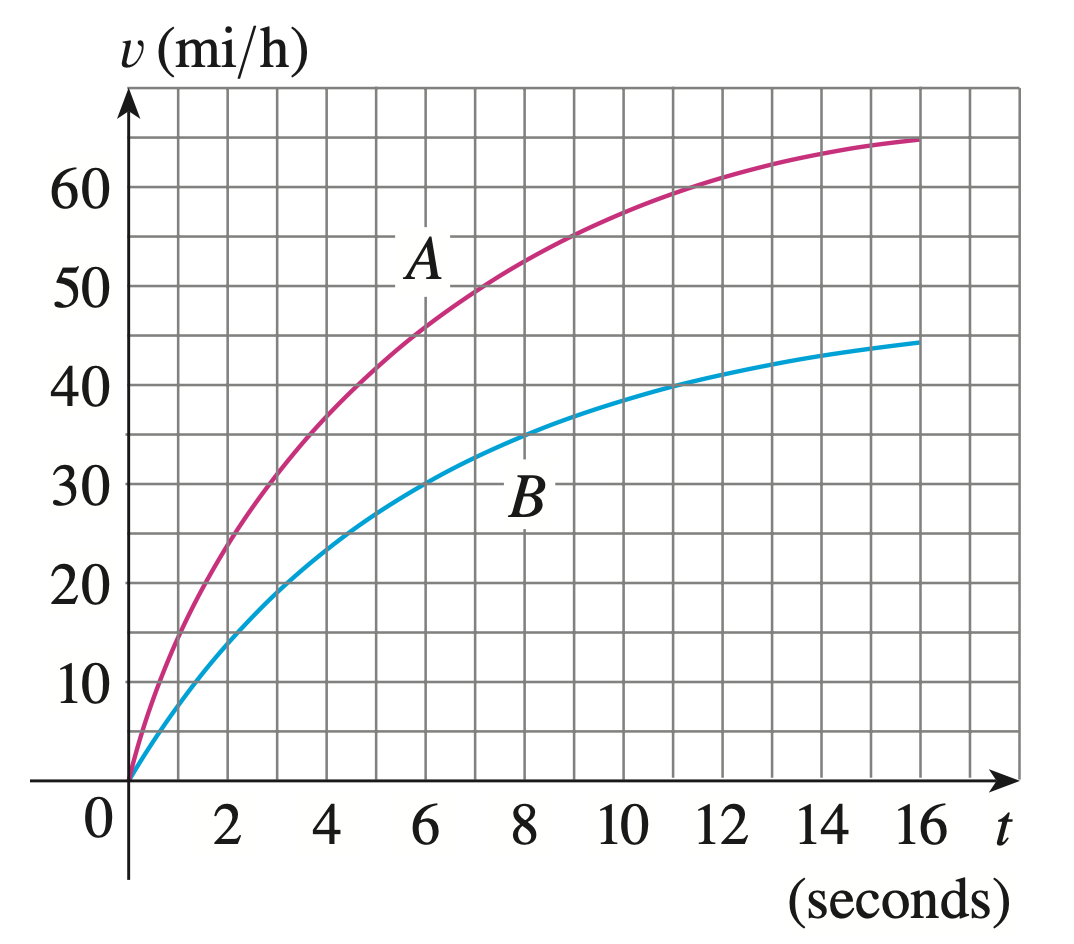
\includegraphics[scale=0.35]{fig/area_case2}
\end{center}
\end{figure}

\end{frame}


\begin{frame}

\frametitle{Example}

Find the area of the region bounded above by $y = e^x$,  bounded below by
$y = x$,  and bounded on the sides by $x = 0$ and $x = 1$

\begin{figure}[t]
\begin{center}
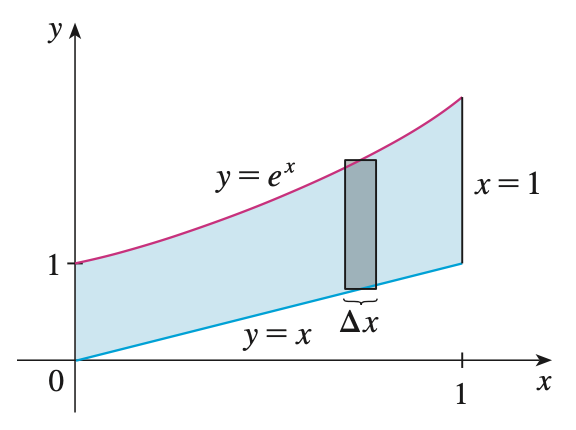
\includegraphics[scale=0.5]{fig/area1}
\end{center}
\end{figure}

\vspace{-2em}

\begin{align*}
A &= \int_{0}^{1} (e^x - x) \, dx = e^x - \frac{1}{2}x^2 \big]_{0}^{1}\\
   &= e - \frac{1}{2} - 1 = e - 1.5
\end{align*}

\end{frame}

\begin{frame}

\frametitle{Example}
\footnotesize
Find the area of the region enclosed by the parabolas $ y = x^2$ and $y= 2x^2 - x^2$

\vspace{-0.5em}
\begin{figure}[t]
\begin{center}
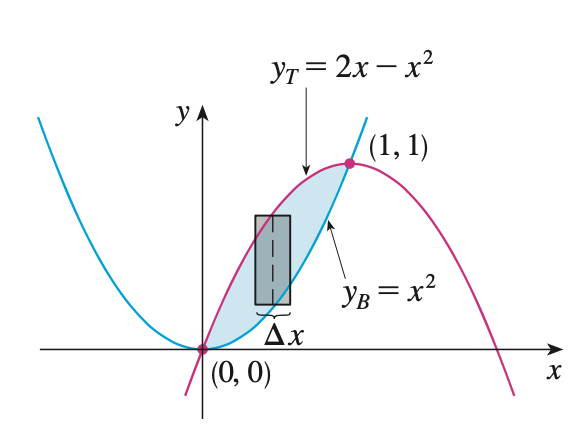
\includegraphics[scale=0.5]{fig/area2}
\end{center}
\end{figure}

\vspace{-1em}

First we need to find the intersection point by solving both equations: $x^2 = 2x - x^2; 2x^2 - 2x = 0; 2x(x-1) = 0; x = 0, 1$.   Thus the intersections points are (0, 0) and (1, 1).

\begin{align*}
A &= \int_{0}^{1} (2x - x^2 - x^2) \, dx = 2  \int_{0}^{1} (x - x^2) \, dx \\
   &= 2\left[ \dfrac{x^2}{2} - \dfrac{x^3}{3}\right]_{0}^{1}= \dfrac{1}{3}
\end{align*}

\end{frame}

\begin{frame}

\frametitle{Exercise}

Find the area of the region enclosed by $y= e^x$ and $y = x^2 - 1$,  with the interval of $x = -1$ and $x=1$ \pause

\begin{align*}
A &= \int_{-1}^{1} (e^x - (x^2 - 1)) \, dx \\
   &= e^x - \frac{1}{3}x^3 + x \big]_{-1}^{1}\\
   &= e - \frac{1}{e} + \frac{4}{3}
\end{align*}

\end{frame}

\begin{frame}

\frametitle{Example}
\footnotesize
Find the area enclosed by the line $y = x - 1$ and the parabola
$y^2 = 2x + 6$

\vspace{-0.5em}
\begin{figure}[t]
\begin{center}
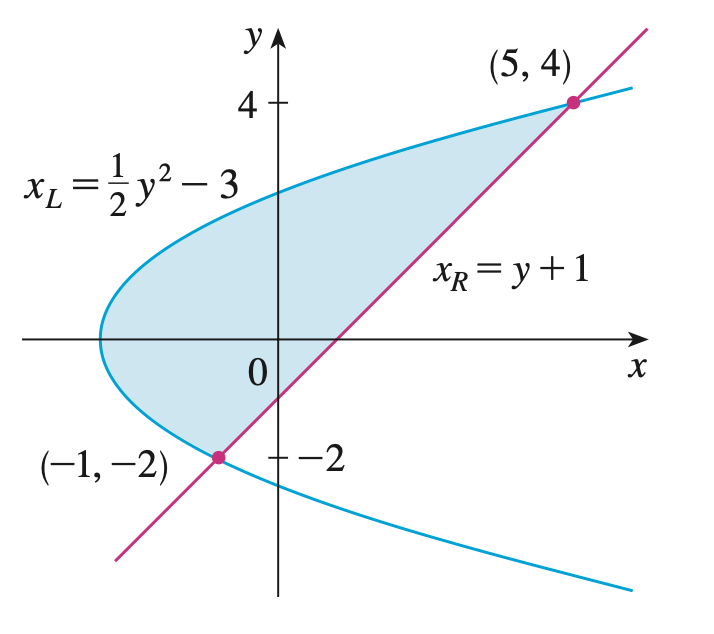
\includegraphics[scale=0.4]{fig/area3}
\end{center}
\end{figure}

\vspace{-2em}

\begin{align*}
A &= \int_{-2}^{4} ((y + 1) - (\frac{1}{2}y^2 - 3)) \, dy \\
   &= \int_{-2}^{4} (-\frac{1}{2}y^2 + y + 4) \,dy = -\dfrac{1}{2}(\dfrac{y^3}{3}) + \dfrac{y^2}{2} + 4y\big]_{-2}^{4} = 18
\end{align*}

\end{frame}

\begin{frame}

\frametitle{Exercise}

Find the area of the region enclosed by $x = 1-y^2$ and $x = y^2 - 1$ with respect to $y$. 

\vspace{-0.5em}
\begin{figure}[t]
\begin{center}
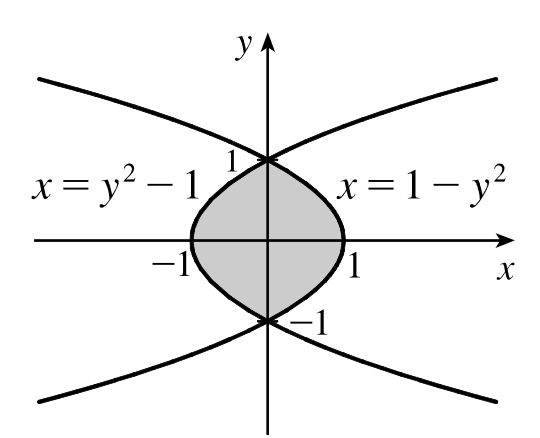
\includegraphics[scale=0.4]{fig/area4}
\end{center}
\end{figure}
\pause
\vspace{-1em}
\begin{align*}
A &= \int_{-1}^{1} ((1-y^2) - (y^2 - 1)) \, dy \\
   &= \int_{-1}^{1} 2(1-y^2) \, dy\\
   &= 2 \cdot \int_{0}^{1} 2(1-y^2) \, dy = \frac{8}{3} \\
\end{align*}

\end{frame}

\section{Average Value}


\begin{frame}
\frametitle{The average value of a function}

\noindent The average value of finitely many numbers $y_1,y_2,\ldots,y_n$ is given by
\[y_{\mathrm{ave}}=\frac{y_1+y_2+\ldots+y_n}{n}.\]
 In general, how do we calculate the average value of a function $y = f(x)$, where $a \leq x \leq b$?
%

\begin{dfn} Suppose that $f$ is continuous on $[a,b]$. Then the \textit{average value} $f_{\mathrm{ave}}$ of $f$ on $[a,b]$ is defined by the formula
\[f_{\textrm{ave}} = \frac{1}{b-a}\int_{a}^{b}f(x)\, dx.\]
The average value is sometimes denoted by $\overline{f}$.\end{dfn}

\end{frame}

\begin{frame}
\frametitle{Example}
Find the average value of the function $f$ over $[-1,2]$, where $f(x)=1+x^2$ \pause

\begin{align*}
f_{\textrm{ave}} &= \frac{1}{b-a}\int_{a}^{b}f(x)\, dx\\
	                         &= \frac{1}{2-(-1)}\int_{-1}^{2}(1 + x^2) \,dx\\
	                         &= \frac{1}{3}\left[x + \frac{x^3}{3} \right]^{2}_{-1}\\
	                         &=2
\end{align*}

\end{frame}

\begin{frame}
\frametitle{Exercise}
Find the average value of the function $f$ over $[-1,2]$, where $f(x)=3x^2 + 8x$ \pause

\begin{align*}
f_{\textrm{ave}} &= \frac{1}{b-a}\int_{a}^{b}f(x)\, dx\\
	                         &= \frac{1}{2-(-1)}\int_{-1}^{2}(3x^2 + 8x) \,dx\\
	                         &= \frac{1}{3}\left[x^3 + 4x^2 \right]^{2}_{-1}\\
	                         &=\frac{1}{3}\left[(8 + 16) - (-1 +4) \right]\\
	                         &=7
\end{align*}

\end{frame}

\begin{frame}
\noindent Suppose that $T(t)$ is the temperature (in ${}^{\circ}$C) at time $t$ (in hours) and that $T_{\mathrm{ave}}$ is the average temperature on the time interval $[0,24]$. Is there a specific time $t_0$ in $[0,24]$ when the temperature $T(t_0)$ is equal to the average temperature $T_{\mathrm{ave}}$?  More generally, given a function $f$, is there a specific value $c$ for which $f(c)=f_{\mathrm{ave}}$?  The answer is yes!  This is called the mean value theorem for integrals.

\begin{theorem}[The Mean Value Theorem for integrals]
If $f$ is continuous on $[a,b]$, then there exists a number $c$ in $[a,b]$ such that
\[f(c) = f_{\textrm{ave}} = \frac{1}{b-a}\int_{a}^{b}f(x)\,dx,\]
that is,
\[ \int_{a}^{b}f(x)\,dx = f(c)(b-a).\]
\end{theorem} 

\end{frame}

\begin{frame}

\frametitle{Mean Value Theorem for Integrals}

\begin{figure}[t]
\begin{center}
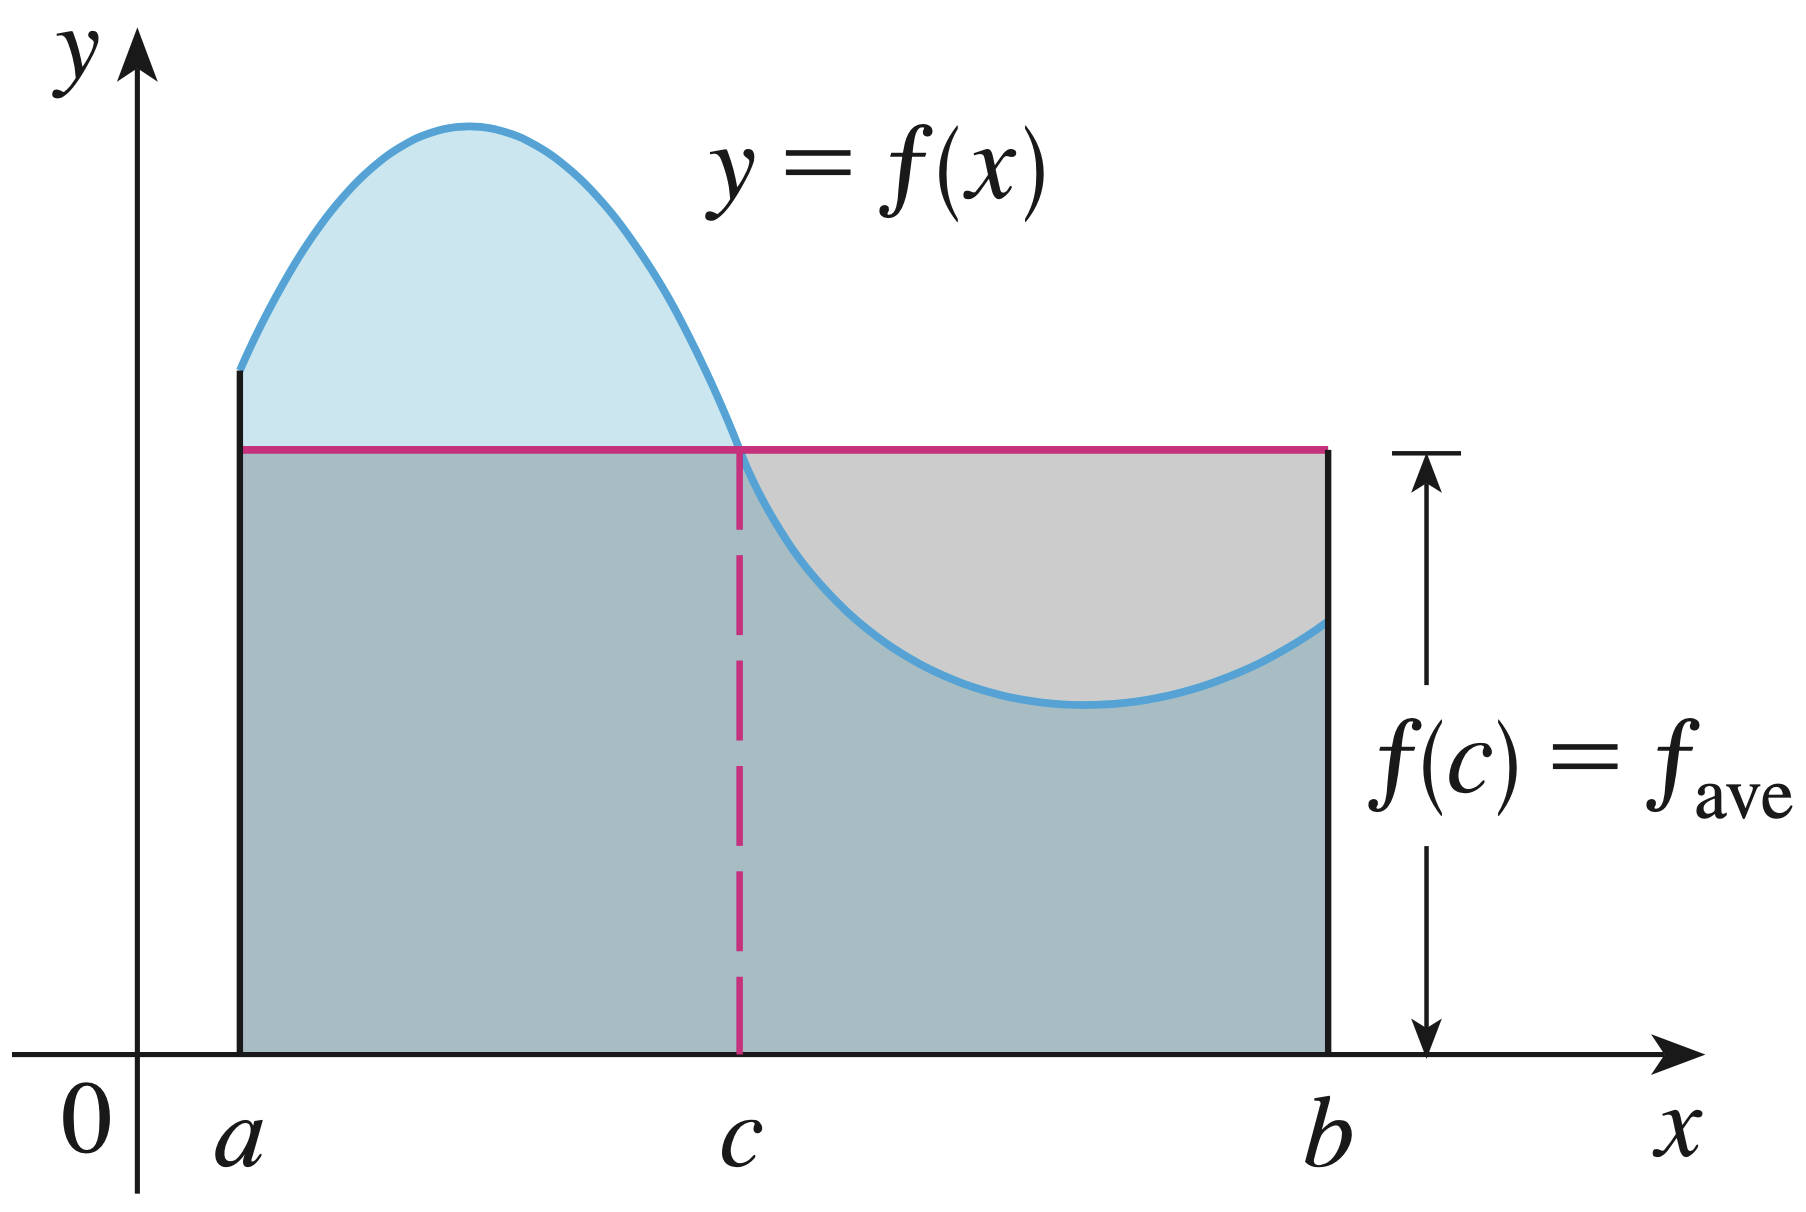
\includegraphics[scale=0.25]{fig/mvt2}
\end{center}
\end{figure}

\end{frame}

\begin{frame}

\frametitle{Example}

Find all numbers $c$ that satisfy the conclusion of the MVT for integrals when $f(x)=1+x^2$ and $[a,b]=[-1,2]$. \pause
\medskip

First, we will find the average value:
\begin{align*}
f_{\textrm{ave}} = \frac{1}{2-(-1)}\int_{-1}^{2}(1 + x^2) \,dx = 2
\end{align*}

Thus, $f(c) = f_{\textrm{ave}} = 2$

\medskip

Then,  we set the $f(c) = 2$, where $f(c) = 1 + c^2$, and solve for $c$:

\begin{align*}
1 + c^2 &= 2\\
          c & \pm 1
\end{align*}

\end{frame}

\begin{frame}

\frametitle{Exercise}

Find all numbers $c$ that satisfy the conclusion of the MVT for integrals when $f(x)=(x - 3)^2$ and $[a,b]=[2,5]$. \pause
\medskip

First, we will find the average value:
\begin{align*}
f_{\textrm{ave}} &= \frac{1}{5-2}\int_{2}^{5}(x-3)^2 \,dx\\
                             &= \frac{1}{3}\left[\frac{1}{3}(x - 3)^3\right]_{2}^{5} = 1\\
\end{align*}

\vspace{-1em}
Thus, $f(c) = f_{\textrm{ave}} = 1$

\medskip

Then,  we set the $f(c) = 1$, where $f(c) = (c - 3)^2$, and solve for $c$:

\vspace{-1em}
\begin{align*}
(c - 3)^2 &= 1\\
        c -3 &= \pm 1\\
        c &= 2 \text{ or } 4\\
\end{align*}

\end{frame}
\end{document}